\documentclass[a4paper,11pt,dvipdfmx]{ujarticle}
% パッケージ
\usepackage{graphicx}
\usepackage{url}
% レイアウト指定を記述したファイルの読み込み
\input{layout}

% タイトルと氏名を変更せよ.
\title{日本におけるデジタル化の状況}
\author{G5848320205 牧 優斗}

\begin{document}

\maketitle %ここにタイトルが入る

% ここから本文
% 節見出し: \section{}
\section{ブロードバンドの整備状況}

% を使う

% 本文(1)
OECDによるブロードバンド回線の普及に関する調査\cite{oecd}によると,図\ref{fig:加入率}に示すように,日本における100人あたりの光ファイバー回線加入者数は29.0で,韓国,スウェーデン,ノルウェーに続いて第4位になっている.
%  参考文献の参照: \cite{}

%  図番号の参照: \ref{}

% を使う
% 文献データベースのキーワードは oecd と imd
% になっている.

% 図の挿入
% \includegraphics{}
\begin{figure}[htbp]
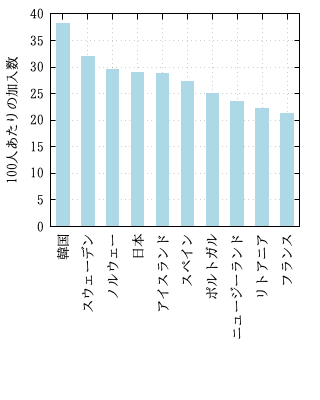
\includegraphics{fig11.png}
\centering
\caption{光ファイバー回線加入者数(100人あたり)}\label{fig:加入率}
\end{figure}
% を
% \begin{figure}[htbp]
% \end{figure}
% で囲み
% \caption{}
% で図のタイトルを入れる.
% \label{}
% を使って図番号が参照できるようにする
% また,
% \centering
% で図が中央に来るようにする

% ーーー
% 節見出し(2)
\section{デジタル競争ランキング}
% 本文(2)
国際経営開発研究所(IMD)の調査\cite{imd}によると,日本のデジタル競争力のランキングは表\ref{tbl:ランキング}に示すように,調査対象の64カ国中,総合で28位,準備分野で27位となっている.
% 表の挿入
% \begin{tabular}
% \end{tabular}    

\begin{table}[htbp]
        \centering
    \caption{デジタル競争力ランキング(64カ国中)}
    \label{tbl:ランキング}
    \begin{tabular}{|c|c|c|}
        \hline
        国 & 総合 & 準備 \\
        \hline
        米国 & 1位 & 1位 \\
        \hline
        香港 & 2位 & 10位 \\
        \hline
        スウェーデン & 3位 & 6位 \\
        \hline
        デンマーク & 4位 & 2位 \\
        \hline
        シンガポール & 5位 & 11位 \\
        \hline
        \hline
        韓国 & 12位 & 5位 \\
        \hline
        中国 & 15位 & 7位 \\
        \hline
        \hline
        日本 & 28位 & 27位 \\
        \hline
    \end{tabular}
\end{table}
% による表の記述を 
% \begin{table}[htbp]
% \end{table}
% で囲み
% \caption{}
% で表のタイトルを入れる.
% \label{}
% を使って表番号が参照できるようにする
% また,
% \centering
% で表が中央に来るようにする

% ーーー
% 見出し(3)
\section{考察}
% 考察

\begin{itemize}
    \item 日本は光ファイバーが世界でもトップクラスに普及している。ため市民生活の中に光ファイバーを用いた通信が溶け込んでいると考えられる。
    \item デジタル競争ランキングは中間あたりに属している。どちらのランキングも変化が少ないため今後デジタル競争力はそのままを維持すると考えられる。
\end{itemize}

% \begin{itemize}
% \end{itemize}
% を使って箇条書きで記述する

% ここに参考文献が入る

\bibliographystyle{junsrt}
\bibliography{exercise.bib}

\end{document}